
\begin{figure*}
 \centering 
    \begin{subfigure}[t]{1.3in}
        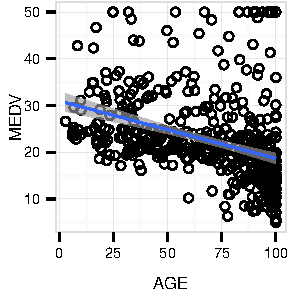
\includegraphics[width=1.3in]{images/AGE-MEDV.pdf}
        \caption{Input scatterplot}
        \label{fig:method_original}
    \end{subfigure}
    \begin{subfigure}[t]{1.5in}
  	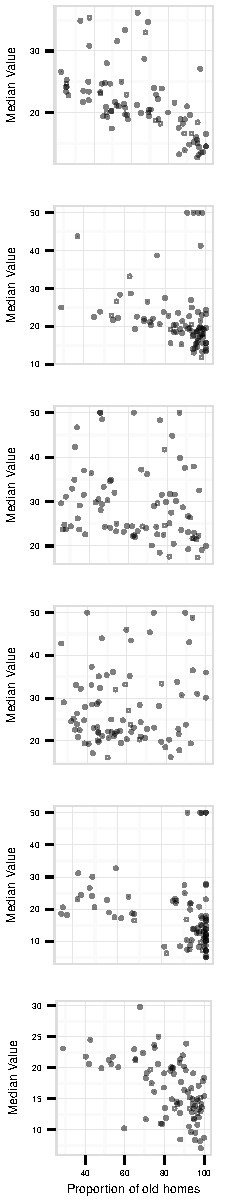
\includegraphics[width=1.5in]{images/DIS.pdf}
	\caption{Partitioned by distance to an\\ employment center}
	 \label{fig:method_actual}
    \end{subfigure}
    \begin{subfigure}[t]{1.5in}
 	 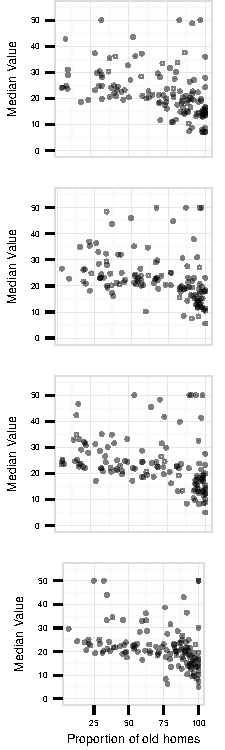
\includegraphics[width=1.5in]{images/randCluster.pdf}
     \vspace{-0.37cm}
 	 \caption{Partitioned by random permutation}
	 \label{fig:method_random}
    \end{subfigure}
     \begin{subfigure}[t]{2.5in}
 	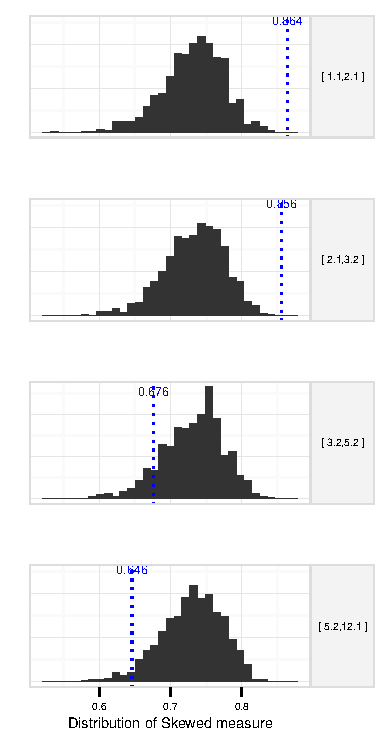
\includegraphics[width=2.5in]{images/hist-DIS.pdf}
	\caption{Distribution of Skewed scagnostics}
	 \label{fig:method_dist}
     \end{subfigure}
   \caption{Illustration of our method of evaluating small multiple displays. (a) The input scatterplot of interest. (b) Partitions determined by the mean distance to Boston's five employment centers. (c) Randomly permuted partitions of the data. (d) Distribution of Skewed scagnostics for the randomly permuted partitions. The overlaid blue lines are the corresponding true scores of the partitions in (b). The blue lines are outliers, indicating that they likely did not arise due to chance. Our algorithm will score the small multiple display in (b) highly.}
\end{figure*}


\section{Method}
\label{sec:method}

Our algorithm takes three inputs from the analyst:
\begin{enumerate}
\item a scatterplot which the analyst wants to partition into a small multiple display,
\item a scagnostic that measures the presence or absence of a visual pattern of interest to the analyst, and
\item a list of potential partitioning variables.
\end{enumerate}
The output is a scoring of the small multiple displays produced by each partitioning variable.

To motivate our algorithm, we first describe four intuitive criteria for effective small multiple displays. We then describe an algorithm that incorporates these criteria to automatically score potential partitioning variables. 

\subsection{Goodness-of-Split Criteria}
We hypothesize that effective small multiple displays conform to the following four criteria:
\begin{itemize}
\item \emph{Visually rich}: Effective small multiple displays should leverage the capabilities of the human visual system by conveying rich visual patterns. This visual richness is unlikely to be captured by the relatively simple summary statistics used in common analytic methods such as ANOVA.

\item \emph{Informative}: Small multiple displays should be more informative than the input visualization, allowing the analyst to deepen their understanding of the data. Small multiple displays that randomly partition the input data are not useful since they contain no more information than the original plot.

\item \emph{Well-supported}: For some data sets, particularly those with outliers or with a small number of data points, strong visual patterns can occur by chance. These spurious patterns are misleading; they appear informative, but are not. Good small multiple displays should convey robust patterns, guiding analysts to reliable results.

\item \emph{Parsimonious}: A small multiple display with many partitions can be very difficult to read and understand. All things being equal, we should favor fewer partitions.
\end{itemize}

\subsection{Algorithm}

The key insight of this paper is that these four criteria can be achieved using a simple heuristic: select small multiple displays that have cognostic values that are unlikely to be due to chance. Using a cognostic to evaluate the small multiple displays ensures that we can find \emph{visually rich} patterns. If the cognostic values are different from that of the input plot, then the small multiple is \emph{informative}. If those differences are unlikely to be due to chance, then it is \emph{well-supported}. And if there are redundant partitioning variables, this heuristic will lead to picking the most \emph{parsimonious}. 

The key challenge in our approach is determining the likelihood of a small multiple display's cognostic value. This is difficult because the underlying distribution of the cognostic score depends on both the cognostic algorithm itself and on the dataset, so we cannot evaluate the likelihood with a closed form formula. Instead, we propose computing this likelihood using a \emph{randomized permutation test}~\cite{Good2000}, which is a non-parametric statistical significance test. This procedure builds an empirical approximation of the underlying cognostic distribution by repeatedly permuting the partitioning variable randomly and computing cognostic values for these random partitions.

To demonstrate how this approach works, consider
Figure~\ref{fig:method_original} which shows the relationship between the median value of owner-occupied houses (in thousands of US dollars) and the proportion of such houses built prior to 1940 for census tracts in the area of Boston, Massachusetts~\cite{Harrison1978}. We see that as the proportion of older houses increases, the median value decreases. However, the distribution is skewed and an analyst may wonder if partitioning this scatterplot by another variable in the dataset that might reveal more about this relationship.
To do so, they run our algorithm using Wilkinson et al.'s \emph{Skewed} scagnostic which can detect a wide range of skewed patterns in scatterplots.

For each possible partitioning variable, we need to compute how unlikely it is that the resulting \emph{Skewed} values are due to chance. For example, consider the ``distance to employment center'' variable shown in Figure~\ref{fig:method_actual}. This variable produces a small multiple display with four plots, one for each quartile of the distance from the census tract to the nearest employment center. Visually we can see that the top two plots are quite skewed and this is verifed by the \emph{Skewed} scagnostic which produces values of 0.864 and 0.856 for the top two plots, but only 0.676 and 0.646 for the bottom two plots. These values are indicated with blue lines in  Figure~\ref{fig:method_dist}.

Next, to evaluate how unlikely it is that these scores arose due to chance, we randomly permute the assignment of data points to partitions, resulting in Figure~\ref{fig:method_random}. Visually the strong skewness of the top two plots has decreased. This indicates that the true scores are probably not just due to chance. If we randomly permute the data set 1000 times, computing the \emph{Skewed} values for each permutation, we can construct the histograms showed in Figure~\ref{fig:method_dist} which show the likelihood that a particular \emph{Skewed} score will occur by chance for each component plot of the small multiple.

By comparing the true \emph{Skewed} values (blue lines) to the random results (black histograms), we can see that the top two plots are in fact more skewed than nearly all the random permutations. Further, the bottom two plots are less skewed than many random permutations. This provides strong evidence that the visual patterns seen in Figure~\ref{fig:method_actual} are not just due to chance, but are rich, informative, and well-supported patterns.  In this case, the small multiple display offers a visual explanation of the relationship between employment center locations to the neighborhoods in Boston---areas with older, lower-valued homes are close to employment centers while newer, higher-valued homes tend to be further away.

To compare this partitioning variable to others, we have to summarize this information into a single score. We first need to summarize how unlikely each component plot is. A straightforward non-parametric way to do this would be with order statistics (a count of how many of the random \emph{Skewed} values were more extreme than the true values). However, in practice we found that often the true value would lay well outside the range of the empirical random distribution. To generate useful likelihood values in these cases would require fitting an analytic distribution to the data. But we also want our approach to work with any cognostic measure, thus we have no a priori information about what analytic distribution we should use. So, instead we use Chebyshev's inequality which can give us a very conservative bound on the likelihood with only weak assumptions about the underlying distribution. This bound is inversely proportional to the standard z-score, so minimizing the likelihood is equivalent to maximizing the absolute z-score:
$$|z_i| = \left|\frac{(X_i-\mu_i)}{\sigma_i}\right|$$ 
where $X_i$ is the true cognostic value of the $i$-th partition and $\mu_i$ and $\sigma_i$ are the mean and standard deviation of the cognostic measures over the repeated random permutations of the $i$-th partition.

Finally, to get a score for the whole small multiple display, we use the maximum absolute z-score across all component plots: 
$$z = \max_{i} |z_i|$$
Using the maximum will result in high scores for small multiple displays that have strong, interesting patterns in at least one component plot. This worked well in our experiments.
%However, it may discount small multiple displays with weaker patterns in many or all the component plots. This is discussed more in Section~\ref{sec:discussion}. 

%Our algorithm will iterate through the twelve possible partitioning variables in this data set, scoring each one. Figure~\ref{fig:method_actual} shows the small multiple display resulting from partitioning on the binned distance to an employment center, one of the variables in the data set. Notice that, compared to the original plot, the density of the top two plots (representing shorter distances to an employment center) appears substantially shifted to the right. While the bottom two plots (longer distances to an employment center) are shifted to the left. These differences will result in Skewed scagnostics that are substantially different from the original plot. 

%However, it is possible that these shifts may have arisen due to random chance. Thus, our algorithm randomly permutes the values of the partitioning variable, producing the small multiple display in Figure~\ref{fig:method_random}. These plots show no sign of the change in skewness and look similar to the original plot. 
%Our algorithm does this repeatedly, producing a distribution of possible random Skewed scagnostic values. In Figure~\ref{fig:method_dist} we show the result of this process with $1000$ repeated simulations. We experimented with increasing the number of simulations with limited gain in stability of the null distribution but with a greater cost to the computational performance. The black histograms show the distribution of the Skewed scagnostic for the random permutations. The blue lines show the Skewed scagnostic for the actual variable---the distance to employment center. For the top two plots, the blue line is to the right of the histogram, indicating that the skewness of these two plots is much higher than we would expect to occur by chance. The bottom two have lower skewness than we would expect by chance, but the values are inside the simulated distribution, so there's less evidence for them.

%After computing z-scores for these four distributions, we use the maximum absolute z-score as the overall score for this small multiple display. This partitioning variable, distance to employment center, is the highest rated in this data set and would be recommended to the analyst.
